


\section{R\'esolution de syst\`eme lin\'eaire}
{\co Comme nous l'avons vu, le calcul des it\'er\'es passe par la r\'esolution de syst\`emes lin\'eaires.} Dans l'exemple de Newton,
 il faut r\'esoudre $\nabla^2 f(x)d_N=\nabla f(x)^T$ o\`u $\nabla^2 f(x^*)\in \mathbb{R}^{n\times n}$
 est une matrice sym\'etrique et $\nabla f(x)^T \in \mathbb{R}^n$.
Il s'agit donc d'un syst\`eme lin\'eaire de la forme $Ax=b$ de grande taille. Il n'est pas envisageable 
d'adopter une r\'esolution du type Cramer, pour que ce soit efficace, nous devons
 modifier la matrice $A$, il existe plusieurs d\'ecompositions:
{\co 
\subsection{Survol des d\'ecompositions classiques pour la r\'esolution}}
\begin{description}
  \item[\'Elimination de Gauss-Jordan] \hfill \\
Aussi appel\'e pivot de Gauss, elle s'applique sur une matrice $A \in \mathbb{R}^{n\times n}$ non singuli\`ere.
 La strat\'egie est de r\'eduire gr\^ace aux op\'erations \'el\'ementaires sur les colonnes de $A$ pour obtenir une matrice triangulaire sup\'erieure. 
Il y a $n-1$ \'etapes, premi\`erement, $A^{(1)}\leftarrow A$ et $b^{(1)}\leftarrow b$ sont initialis\'es. Au bout
de la $k$i\`eme \'etape, nous avons $A^{(k)}x=b^{(k)}$ %o\`u
$$A^{(k)}= \left[
\begin{array}{rl}
 A^{(k)}_{11} & A^{(k)}_{12} \\
 0       & A^{(k)}_{22} \\
\end{array}\right]$$
o\`u $A^{(k)}_{11} \in \mathbb{R}^{(k-1)\times(k-1)}$ est une matrice triangulaire sup\'erieure.

L'\'elimination de Gauss-Jordan a un coût de $\frac{2}{3}n^3$.


  \item[D\'ecomposition LU] \hfill \\
Pour une matrice $A\in \mathbb{R}^{n\times n}$, cette d\'ecomposition fournit deux matrices $LU$ o\`u
$L$ est une matrice triangulaire inf\'erieure et $U$ une matrice triangulaire sup\'erieure. Il existe une unique d\'ecomposition si
et seulement si $A_k=A(1:k,1:k)$ est non singuli\`ere pour $k=1:n-1$, sinon elle existe mais n'est pas unique.

La d\'ecomposition LU a un coût de l'ordre de $\frac{2}{3}n^3$.


  \item[D\'ecomposition de Cholesky] \hfill \\


Cette d\'ecomposition, dûe au fran\c{c}ais Andr\'e-Louis Cholesky (1875-1918 alors qu'il \'etait commandant en chef) permet de r\'esoudre de mani\`ere efficace des syst\`emes
 d'\'equation lin\'eaire de la forme $Ax=b$ lorsque $A$ est une matrice d\'efinie positive.

\begin{frtheoreme}
 Si A est une matrice r\'eelle sym\'etrique,  d\'efinie positive, alors il existe une unique matrice L
triangulaire inf\'erieure et inversible, telle que
 $$A = LL^T$$
\end{frtheoreme}



\begin{algorithm}                     % enter the algorithm environment
\caption{Factorisation de Cholesky}          % give the algorithm a caption
\label{alg:chol}                           % and a label for \ref{} commands later in the document
\begin{algorithmic}  
\STATE \textbf{Pr\'ealables:} %Variables en entr\'ee :  
\begin{itemize}
\item[$\bullet$] Soit $A \in \mathbb{R}^{n\times n}$ une matrice sym\'etrique d\'efinie positive
\end{itemize}
\STATE \textbf{En sortie:} %Variables en entr\'ee :  
\begin{itemize}
\item[$\bullet$] calcule $R$ o\`u $A=R^TR$ et $R=(r_{ij})_{1\leq i,j\leq n}$
\end{itemize}
\FOR{$j = 1:n$} 
\FOR{$i = 1:n$} 
\STATE $r_{ij}\leftarrow(a_{ij}-\sum_{k=1}^{i-1}r_{ki}r_{kj})/r_{ii}$
\ENDFOR
\STATE $r_{jj}=(a_{jj}-\sum_{k=1}^{j-1}r_{kj}^2)^{1/2}$
\ENDFOR
\end{algorithmic}
\end{algorithm}


Pour r\'esoudre le syst\`eme, $Ax = LL^Tx = b$, on commence par r\'esoudre $Ly=b$ puis $L^Tx=y$.
Le nombre d'op\'erations requis pour cette d\'ecomposition est de l'ordre de $\frac{1}{3}n^3$. Il s'agit de la m\'ethode 
la plus efficace donc celle que l'on devrait utiliser, cependant lorsque la m\'ethode de Newton est appliqu\'ee,
la matrice hessienne n'est a priori pas d\'efinie positive. C'est pour cette raison que l'algorithme de Cholesky a \'et\'e 
modifi\'e. La matrice va être corrig\'ee pour obtenir une d\'ecomposition d\'efinie positive
 et plutôt bien conditionn\'ee.
\end{description}


\subsection{D\'ecomposition de Cholesky Modifi\'ee}
\label{chap1:decomposition}

Soit une matrice $A$, sym\'etrique mais pas n\'ecessairement d\'efinie positive. L'algorithme de Cholesky modifi\'ee
calcule la d\'ecomposition $P(A+E)P^T=LDL^T$ o\`u $P$ est une matrice de permutation, $E$ est une
perturbation pour rendre la matrice $A+E$ d\'efinie positive, $D$ est une matrice diagonale et 
$L$ une matrice triangulaire inf\'erieure. La norme de $E$ devrait être petite et $A+E$ 
bien conditionn\'ee. Cette technique est largement utilis\'ee en optimisation comme dans notre cas ou bien pour 
calculer des pr\'e-conditionneurs d\'efinis positifs.
Comme le soulignent Cheng et Higham dans \cite{Higham}, les objectifs de l'algorithme de Cholesky modifi\'e peuvent être d\'eclar\'es
comme suit :
\begin{itemize}
\item[O1] Si $A$ est "suffisamment d\'efinie positive", alors $E$ devrait être \'egale \`a z\'ero.
\item[O2] Si $A$ est ind\'efinie, $\lVert E \rVert$ ne devrait pas être plus grand que 
\[\min\{\lVert \Delta A \rVert: A+\Delta A \text{ est d\'efinie positive } \} \]
pour une norme appropri\'ee.
\item[O3] La matrice $A+E$ devrait être raisonnablement bien conditionn\'ee. 
\item[O4] Le coût de l'algorithme devrait être le même que le coût de la d\'ecomposition standard de Cholesky
 pour l'ordre le plus \'elev\'e.
\end{itemize}



  \section{Utilisation de la d\'ecomposition de Cholesky modifi\'ee}

\label{chap3:cholesky}

Il existe plusieurs versions de la d\'ecomposition de Cholesky modifi\'ee en Scilab mais pas 
de version efficace. Cela est li\'e intrins\`equement \`a {\it Scilab} qui est un langage de haut niveau et n'est pas performant pour effectuer du code
imp\'eratif sur des grandes dimensions comparativement au C ou Fortran.
Par cons\'equent, nous avons choisi deux routines appartenant \`a Lapack\footnote{\url{http://www.netlib.org/lapack/}}, une libraire sur les syst\`emes lin\'eaires \'ecrite en fortran.
 La premi\`ere permet la d\'ecomposition 
de Cholesky modifi\'ee et la deuxi\`eme la r\'esolution du syst\`eme avec cette d\'ecomposition, nomm\'ee {\tt dsytrf} et {\tt dsytrs} respectivement. 
Cette d\'ecomposition de Cholesky modifi\'ee utilise la m\'ethode de pivotement de Bunch-Kaufman (BK) \cite{Bunch}.

Soit une matrice $A \in \mathbb{R}^{n\times n}$ non nulle, la factorisation fournit $$P(A+E)P^T=L(D+F)L^T.$$ $F$ est choisie pour que $D+F$ et ainsi
$A+E$ soient d\'efinies positives. Cette technique a \'et\'e propos\'ee par Mor\'e et Sorensen \cite{More}. L'id\'ee consiste \`a 
trouver une permutation $\Pi$ et un entier $s=1$ ou $2$ tel que 

\begin{equation*}
\Pi A \Pi^T = 
\left[
\begin{array}{cc}
 E & C^T \\
 C & B \\
\end{array}\right]
\end{equation*}
avec $E\in \mathbb{R}^{s\times s}$ non singuli\`ere et $B\in \mathbb{R}^{(n-s)\times (n-s)}$. En choisissant correctement $\Pi$, nous avons la factorisation :

\begin{equation*}
\Pi A \Pi^T = 
\left[
\begin{array}{cc}
 I_s & 0 \\
 CE^{-1} & I_{n-s} \\
\end{array}\right]
\left[
\begin{array}{cc}
 E & 0 \\
 0 & B-CE^{-1}C^T \\
\end{array}\right]
\left[
\begin{array}{cc}
 I_s & E^{-1}C^T \\
 0 & I_{n-s} \\
\end{array}\right]
\end{equation*}
Le proc\'ed\'e est r\'ep\'et\'e r\'ecursivement sur la matrice $S=B-CE^{-1}C^T$ de taille\\ $(n-s)\times (n-s)$. On remarque ainsi qu'au lieu
d'utiliser un pivot de taille $1\times 1$, on peut utiliser une matrice $2\times2$.




 Selon Cheng et Higham \cite{Higham}, l'algorithme de BK, que celui de Schnabel et Heskow \cite{choleskymod}, a un coût identique
 \`a la d\'ecomposition de Cholesky standard relativement
aux termes d'ordre les plus \'elev\'es, cependant les objectifs O1 et O3 de la partie \ref{chap1:decomposition} sont difficilement satisfaits.
Il se peut que la matrice $A+E$ soit mal conditionn\'ee car $\lVert L \rVert_{\infty}$ n'est pas born\'ee et par cons\'equent les valeurs propres de $D$ peuvent 
largement diff\'erer de $A$. 
Les auteurs proposent ainsi une autre version de l'algorithme de BK, permettant de satisfaire les conditions mais nous consid\'ererons que 
les routines de lapack permettrons d'obtenir des directions satisfaisantes d'autant plus que nous utiliserons une recherche lin\'eaire ce qui injectera
un niveau de contrôle en plus.

Afin d'obtenir une matrice d\'efinie positive, nous profitons de cette d\'ecomposition pour changer les \'el\'ements diagonaux.
L'avantage, c'est que l'on a plus besoin de faire ces changements sur une matrice $n$ par $n$ mais seulement $2\times2$ ou $1\times1$.

\begin{algorithm}                     % enter the algorithm environment
\caption{Changement de la diagonale}          % give the algorithm a caption
\label{alg:diag}                           % and a label for \ref{} commands later in the document
\begin{algorithmic}
\STATE \textbf{Pr\'ealables:} %Variables en entr\'ee :  
\begin{itemize}
\item[$\bullet$] $\epsilon>0$
\item[$\bullet$] $\Tilde{D}$ la matrice diagonale par bloc
\end{itemize}
\STATE \textbf{Sortie} %Variables en entr\'ee :  
\begin{itemize}
\item[$\bullet$] $D$ la matrice diagonale par bloc avec pour valeur 
propre minimale $\lambda_{min} \geq \epsilon$
\end{itemize}

\STATE Pour chaque bloc de la diagonale $\Tilde{D_k}$,
\IF{$\Tilde{D_k}$ est de dimension $1\times1$}
\STATE $D_k\leftarrow \max(\Tilde{D_k},\epsilon)$
\ELSE 
%\COMMENT{$D$ est de dimension $2\times2$} 
\STATE $[Z,W]=spec(\Tilde{D_k)}$
\COMMENT{Il s'agit de la diagonalisation de $\Tilde{D_k}$ : $ZWZ^T=\Tilde{D_k}$ avec $W$ matrice diagonale}
\STATE $D_k\leftarrow Z*diag(max(diag(W),\epsilon))*Z^T$
\ENDIF
\end{algorithmic}
\end{algorithm}


% function D=moddiag(D,Ipiv)
% [nr,n]=size(D);
% eps=0.00001
% 
% first(1)=%t
% for j=1:n-1
% 	    if(Ipiv(j)<0 & first(j)) then first(j+1)=%f, D(j,j+1)= D(j+1,j)
% 	    else first(j+1)=%t
% 	    end
% end
% for i=1:n
%       if(first(i)) then
% 	  if(Ipiv(i)<0) then
% 	      [Z,W]=spec(D(i:i+1,i:i+1));
% 	      D(i:i+1,i:i+1)=Z*diag(max(diag(W),eps))*Z'
% 	      else D(i,i)=max(D(i,i),eps)
% 	  end
%       end
% end
% endfunction
% eps=0.00001
% A=rand(2,2)
% A=A+A'
% [Z,W]=spec(A)
% A2=Z*diag(max(diag(W),eps))*Z'



\section{R\'esolution des syst\`emes lin\'eaires}

\label{chap2:decomp}
Pour commencer, il est \`a noter que la r\'esolution 
des syst\`emes triangulaires dans {\it Scilab} n'est g\'en\'eralement pas efficace. Il s'av\`ere que la d\'etection du syst\`eme triangulaire 
n'est pas faite syst\'ematiquement. La figure \ref{fig:lu} r\'ev\`ele que sur les quatre tests de r\'esolution
 $Lx=e$, $L'x=e$, $U'x=e$, $Ux=e$ o\`u $L$ et $U$ proviennent de la d\'ecomposition $LU$ r\'ealis\'e par {\it Scilab} et
 $e=(1)_{1\leq i\leq n}$ un vecteur colonne, une seule est performante.

\begin{figure}
\caption{R\'esolution d'un syst\`eme triangulaire par {\it Scilab} avec une d\'ecomposition LU, sur les quatre versions,
qu'une seule n'est efficace.}
\center
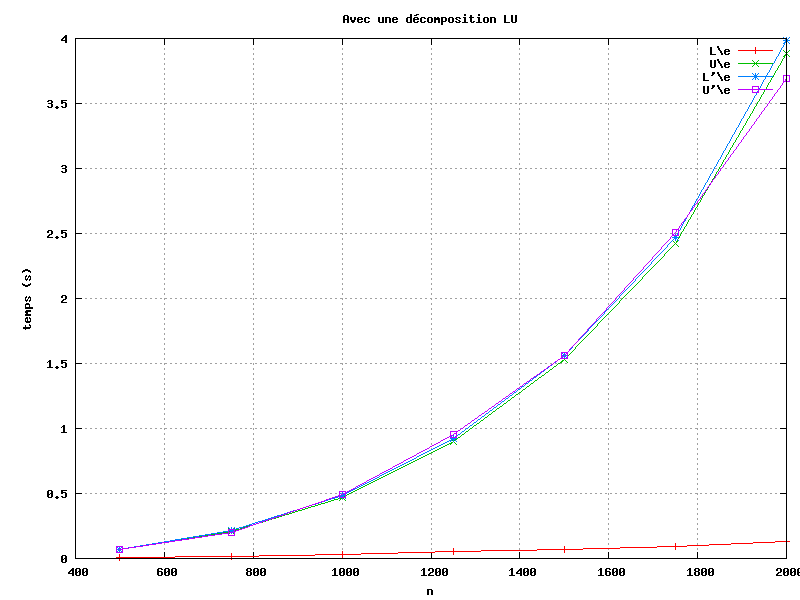
\includegraphics[scale=0.39]{figures/LU.png}
\label{fig:lu}
\end{figure}


\begin{figure}
\caption{R\'esolution d'un syst\`eme triangulaire par {\it Scilab} avec une d\'ecomposition de Cholesky}
\center
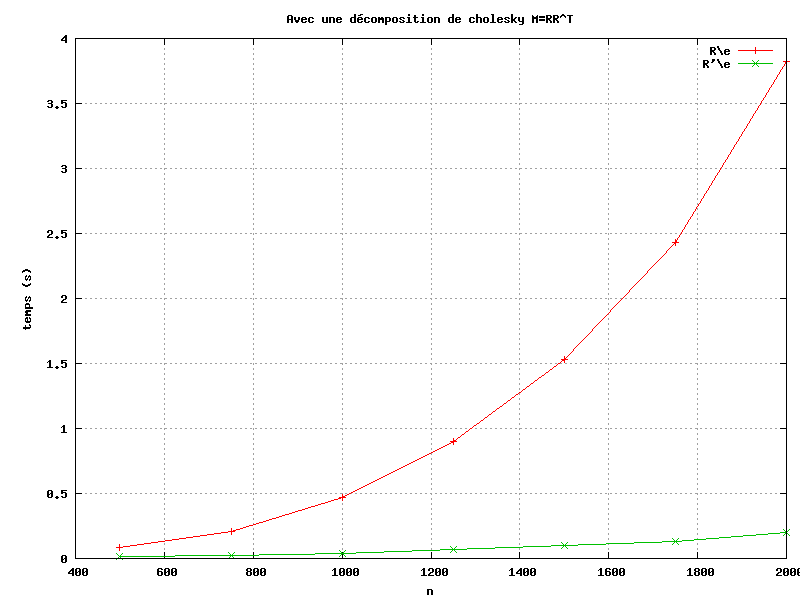
\includegraphics[scale=0.39]{figures/chol.png}
\label{fig:chol}
\end{figure}

C'est pour cette raison que nous avons pr\'ef\'er\'e choisir une d\'ecomposition \'ecrite en fortran pour nos calculs.


La r\'esolution des syst\`emes $Ax=b$ s'effectue en trois temps. Tout d'abord, $A$ qui est par exemple 
la hessienne de notre fonction, est d\'ecompos\'ee en

 $$L\Tilde{D}L^T=P^T(A+E)P$$ o\`u $D$ est une matrice diagonale par bloc soit de taille $1\times 1$, soit $2\times 2$.
 La factorisation a un coût de $\frac{1}{3}n^3$. Ensuite, on modifie chacun de ces blocs
pour le rendre d\'efini positif : $D\leftarrow \Tilde{D}+\Delta \Tilde{D}$. Cette op\'eration est 
de l'ordre de $n$ mais elle est effectu\'ee avec {\it Scilab}
 Enfin, on r\'esout le syst\`eme $LDL^Tx=b$ qui est une op\'eration en $n^2$.








\subsection{Temps de calcul de l'ensemble de la r\'esolution}


Comme le montre la figure \ref{fig:temps8}, la factorisation modifi\'ee est l'op\'eration qui prend le plus de temps,
elle a un comportement en $n^3$. La r\'esolution du syst\`eme lin\'eaire est plus rapide que le changement de la 
diagonale parce qu'elle est ex\'ecut\'ee en fortran.
\begin{figure}
\caption{R\'esolution du syst\`eme $Ax=b$ avec la factorisation de Cholesky modifi\'ee}
\center
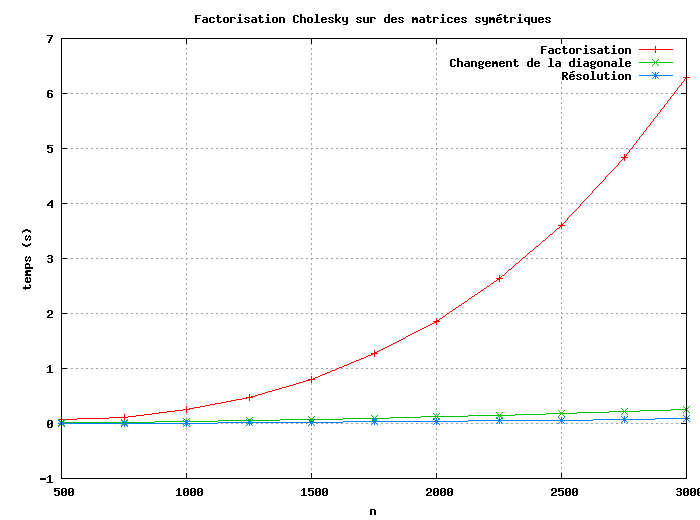
\includegraphics[scale=0.4]{figures/temps8.png}
\label{fig:temps8}
\end{figure}


\begin{table}[h]
	\begin{center}
\begin{tabular}{|c|c|c|c|c|}\hline
n & D\'ecomposition & Arrangement & R\'esolution & $A \backslash b$ avec Scilab\\
 & $A\leftarrow LDL^T$ & $D\leftarrow \Tilde{D}+\Delta \Tilde{D}$& $Lu=b$, $\Tilde{D}v=u$, $L^Tx=v$ & \\
\hline
$500 $&$  0.037000 $&$  0.011000 $&$ 0.002000 $&$ 0.090000$\\\hline
$750 $&$ 0.122000 $&$ 0.026000 $&$ 0.005000 $&$ 0.220000$\\\hline
$1000 $&$ 0.254000 $&$ 0.038000 $&$ 0.010000 $&$ 0.486000$\\\hline
$1250 $&$ 0.475000 $&$ 0.055000 $&$ 0.015000 $&$ 0.944000$\\\hline
$1500 $&$ 0.809000 $&$ 0.075000 $&$ 0.022000 $&$ 1.607000$\\\hline
$1750 $&$ 1.278000 $&$ 0.097000 $&$ 0.030000 $&$ 2.543000$\\\hline
$2000 $&$ 1.863000 $&$ 0.123000 $&$ 0.038000 $&$ 3.732000$\\\hline
$2250 $&$ 2.636000 $&$ 0.149000 $&$ 0.047000 $&$ 5.413000$\\\hline
$2500 $&$ 3.602000 $&$ 0.179000 $&$ 0.057000 $&$ 7.402000$\\\hline
$2750 $&$ 4.830000 $&$ 0.215000 $&$ 0.070000 $&$ 10.116000$\\\hline
$3000 $&$ 6.320000 $&$ 0.251000 $&$ 0.084000 $&$ 13.327000$\\\hline
\end{tabular}
	\end{center}
	\caption{Temps de calcul en seconde pour chaque \'etape de la r\'esolution du syst\`eme $Ax=b$, bien que la modification de la diagonale soit
$\mathcal{O}(n)$, elle est moins efficace que la r\'esolution car elle est cod\'ee en {\it Scilab}.}
	\label{tab:newton}
\end{table}



{\co 
\subsection{Conclusion}
Nous venons d'obtenir une interface reliant {\it Scilab} \`a {\it Fortran} nous permettant d'obtenir
une r\'esolution de syst\`emes lin\'eaire de mani\`ere efficace et ce même si la matrice n'est pas d\'efinie 
positive. 
\`A pr\'esent, nous allons nous interesser \`a la diff\'erentition automatique, les probl\`ematiques qu'elle
soul\`eve et diff\'erents modes qui existent. Nous verrons plus tard si les outils sont suffisamment performants
pour valider les bornes de complexit\'e d\'efinies dans le chapitre 1.
}




